% Copyright (c) 2022 by Lars Spreng
% This work is licensed under the Creative Commons Attribution 4.0 International License.

\documentclass[
11pt,notheorems,hyperref={pdfauthor=whatever}
]{beamer}

\usepackage{kotex}
\input{loadslides.tex}

\usepackage{fontspec}
\IfFileExists{/Users/seojunha/Library/Fonts/NotoSansCJKkr-Regular.otf}{%
  \setmainhangulfont[
    Path=/Users/seojunha/Library/Fonts/,
    BoldFont=NotoSansCJKkr-Bold.otf
  ]{NotoSansCJKkr-Regular.otf}
  \setsanshangulfont[
    Path=/Users/seojunha/Library/Fonts/,
    BoldFont=NotoSansCJKkr-Bold.otf
  ]{NotoSansCJKkr-Regular.otf}
  \setmonohangulfont[
    Path=/Users/seojunha/Library/Fonts/,
    BoldFont=NotoSansCJKkr-Bold.otf
  ]{NotoSansCJKkr-Regular.otf}
}{%
  \IfFontExistsTF{Noto Sans CJK KR}{%
    \setmainhangulfont{Noto Sans CJK KR}
    \setsanshangulfont{Noto Sans CJK KR}
    \setmonohangulfont{Noto Sans CJK KR}
  }{%
    \IfFontExistsTF{NanumGothic}{%
      \setmainhangulfont{NanumGothic}
      \setsanshangulfont{NanumGothic}
      \setmonohangulfont{NanumGothic}
    }{}%
  }%
}
\renewcommand{\familydefault}{\sfdefault}

\definecolor{TextGray}{HTML}{333333}
\definecolor{AccentOrange}{HTML}{08457E}
\definecolor{SoftOrange}{HTML}{EAF0F8}
\definecolor{LineGray}{HTML}{B8B8B8}

\usepackage{tikz}
\usetikzlibrary{arrows.meta, positioning, fit, backgrounds, calc, shapes.geometric}

\addtobeamertemplate{frametitle}{}{\vspace{-0.5em}}

\tikzset{
  box/.style={draw=LineGray, rounded corners=2pt, fill=white, align=center, minimum height=0.82cm, inner sep=5pt, font=\small},
  orangebox/.style={draw=AccentOrange, very thick, rounded corners=2pt, fill=SoftOrange, align=center, minimum height=0.82cm, inner sep=5pt, font=\small\bfseries},
  arrow/.style={-{Latex[length=2.6mm]}, thick, draw=AccentOrange},
  grayarrow/.style={-{Latex[length=2.4mm]}, thick, draw=LineGray}
}

\newcommand{\smallgray}[1]{{\scriptsize\textcolor{gray!75}{#1}}}
\newcommand{\smallred}[1]{{\scriptsize\textcolor{red!70!black}{#1}}}
\newcommand{\tagbox}[1]{\colorbox{SoftOrange}{\strut\scriptsize #1}}
\newcommand{\yes}{\textcolor{TextGray}{Yes}}
\newcommand{\no}{\textcolor{TextGray}{No}}

\setbeamerfont{title}{size=\LARGE,series=\bfseries}
\setbeamerfont{subtitle}{size=\normalsize}
\setbeamerfont{frametitle}{series=\bfseries}

\title[]{LLM-Based Sequential Clinical Diagnosis}
\subtitle{Recent Progress and Open Challenges}
\author[]{SeoJun Ha}
\institute{DGIST}
\date{May 22, 2026}

\begin{document}

{
\setbeamertemplate{footline}{}
\begin{frame}
  \titlepage
  \vspace{-0.8em}
  \begin{center}
  \scriptsize
  LA-CDM · LDTL · SIFT · CaRT · MIMIC-CDM
  \end{center}
\end{frame}
}
\addtocounter{framenumber}{-1}

\begin{frame}{Survey Map}
\vspace{0.45em}
\begin{center}
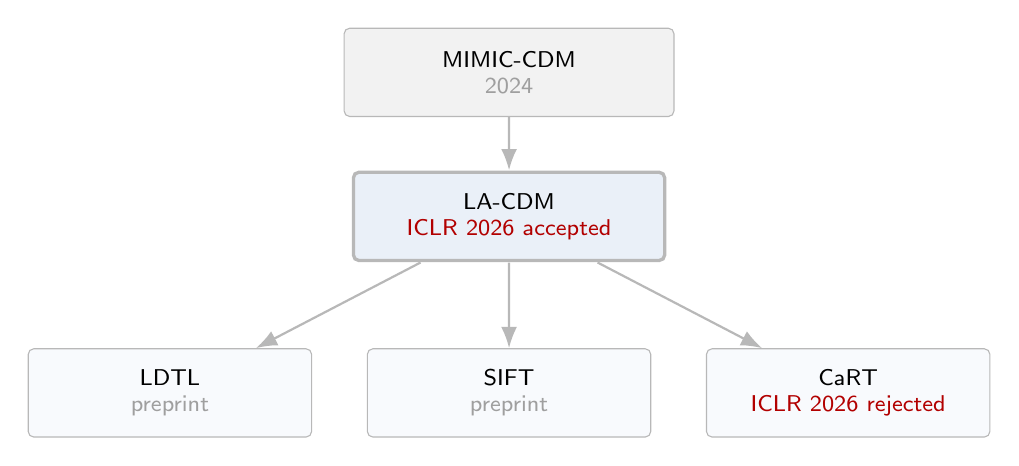
\begin{tikzpicture}[scale=1.18, transform shape,
  paper/.style={draw=LineGray, rounded corners=2pt, fill=white, align=center, minimum width=3.05cm, minimum height=0.95cm, font=\scriptsize},
  root/.style={paper, fill=gray!10, minimum width=3.55cm},
  hub/.style={paper, draw=LineGray, very thick, fill=SoftOrange, minimum width=3.35cm},
  axis/.style={font=\scriptsize\bfseries, text=TextGray}
]
\node[root] (data) at (0,0) {MIMIC-CDM\\\smallgray{2024}};
\node[hub] (lacdm) at (0,-1.55) {LA-CDM\\\smallred{ICLR 2026 accepted}};
\node[paper, fill=SoftOrange!35] (ldtl) at (-3.65,-3.45) {LDTL\\\smallgray{preprint}};
\node[paper, fill=SoftOrange!35] (sift) at (0,-3.45) {SIFT\\\smallgray{preprint}};
\node[paper, fill=SoftOrange!35] (cart) at (3.65,-3.45) {CaRT\\\smallred{ICLR 2026 rejected}};

\draw[-{Latex[length=2.7mm]}, thick, draw=LineGray] (data) -- (lacdm);
\draw[-{Latex[length=2.7mm]}, thick, draw=LineGray] (lacdm) -- (ldtl);
\draw[-{Latex[length=2.7mm]}, thick, draw=LineGray] (lacdm) -- (sift);
\draw[-{Latex[length=2.7mm]}, thick, draw=LineGray] (lacdm) -- (cart);
\end{tikzpicture}
\end{center}
\vspace{-0.1em}
\begin{block}{Recently Emerging Problem Setting}
\small
MIMIC-CDM (2024) introduced \textbf{sequential evidence acquisition} as a benchmark,
shifting LLM diagnosis from ``full-information classification'' to learning ``which test to inspect and when.''
\end{block}
\end{frame}

\begin{frame}{Main Focus}
\vspace{0.55em}
\begin{block}{What is a good trajectory?}
\small
We have the ground-truth diagnosis label, but \textbf{we do not have labels for good diagnostic paths}. Recent studies therefore fill this gap with different proxies, without directly observing the optimal trajectory.
\end{block}

\vspace{0.9em}
\begin{center}
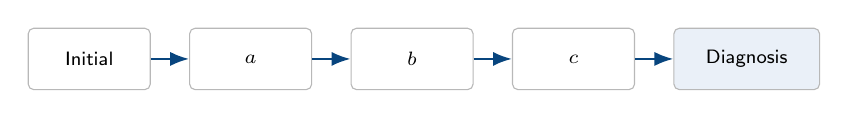
\begin{tikzpicture}[
  trajnode/.style={draw=LineGray, rounded corners=2pt, fill=white, align=center, minimum width=1.55cm, minimum height=0.78cm, font=\scriptsize},
  trajarrow/.style={-{Latex[length=2.4mm]}, thick, draw=AccentOrange}
]
\node[trajnode] (init) at (0,0) {Initial};
\node[trajnode] (a) at (2.05,0) {\(a\)};
\node[trajnode] (b) at (4.10,0) {\(b\)};
\node[trajnode] (c) at (6.15,0) {\(c\)};
\node[trajnode, minimum width=1.85cm, fill=SoftOrange] (diag) at (8.35,0) {Diagnosis};

\draw[trajarrow] (init) -- (a);
\draw[trajarrow] (a) -- (b);
\draw[trajarrow] (b) -- (c);
\draw[trajarrow] (c) -- (diag);
\end{tikzpicture}
\end{center}
\end{frame}

\begin{frame}{MIMIC-CDM Dataset}
\vspace{0.15em}
\begin{columns}[T,onlytextwidth]
\begin{column}{0.45\textwidth}
\begin{block}{Benchmark Goal}
\small
Instead of a classification task where all patient information is given at once, MIMIC-CDM defines a clinical decision-making benchmark where the model must \textbf{select tests sequentially} and then predict the diagnosis.
\end{block}

\vspace{0.35em}
\begin{block}{Scale and Labels}
\small
A total of \textbf{2,400} abdominal disease patient cases.

\vspace{0.35em}
\textbf{Disease list}
\begin{itemize}
\item appendicitis
\item cholecystitis
\item diverticulitis
\item pancreatitis
\end{itemize}
\end{block}
\end{column}

\begin{column}{0.51\textwidth}
\begin{block}{Action space: 12 actions}
\small
\textbf{1. Lab tests} \hfill {\footnotesize 7 actions}

\vspace{0.15em}
{\footnotesize
Complete Blood Count, Basic Metabolic Panel, Comprehensive Metabolic Panel, Renal Function Panel, Liver Function Panel, Urinalysis, Electrolyte Panel
}

\vspace{0.65em}
\textbf{2. Imaging reports} \hfill {\footnotesize 4 actions}

\vspace{0.15em}
{\footnotesize CT, MRI, Radiograph, Ultrasound}

\vspace{0.65em}
\textbf{3. Physical examination} \hfill {\footnotesize 1 action}

\vspace{1.0em}
{\footnotesize\textcolor{red}{Some patients do not have records for certain test results.}}
\end{block}
\end{column}
\end{columns}
\end{frame}

\begin{frame}[plain]
\centering
\vspace{0.22\textheight}
{\Large\bfseries Language Agents for Hypothesis-driven\\Clinical Decision Making with Reinforcement Learning}
\vspace{1.2em}

{\small LA-CDM}\\
{\scriptsize ICLR 2026}
\end{frame}

\begin{frame}{LA-CDM: Motivation}
\vspace{0.1em}
\begin{block}{1. Existing clinical RL mostly focuses on tabular data}
\small
Prior reinforcement-learning approaches to clinical decision-making are mostly designed for \textbf{tabular data}. As a result, they miss clinically important modalities such as clinical notes and imaging reports.
\end{block}

\vspace{0.55em}
\begin{block}{2. Existing LLM clinical decision-making is mostly zero-shot}
\small
Existing LLM-based clinical decision-making mostly relies on prompting or zero-shot reasoning. It does not explicitly train \textbf{diagnostic test selection or sequential decision-making itself}.
\end{block}

\vspace{0.55em}
\begin{block}{LA-CDM Problem Setting}
\small
LA-CDM frames LLM-based clinical decision-making as sequentially requesting tests from a multimodal patient state and making a diagnosis when confidence is sufficient.
\end{block}
\end{frame}

\begin{frame}{LA-CDM: Main Figure}
\centering
\vspace{0.2em}
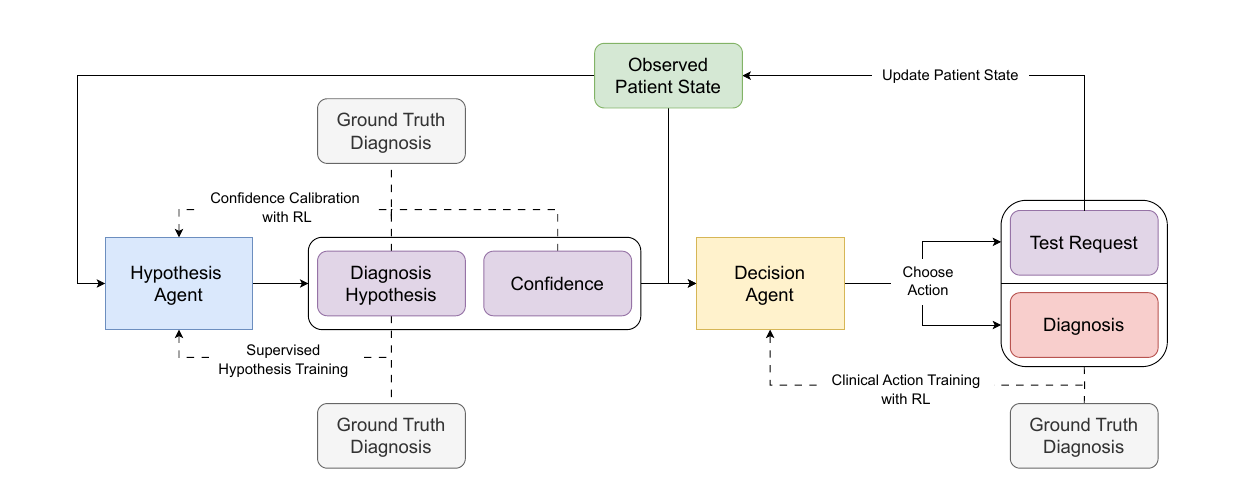
\includegraphics[width=0.98\linewidth,height=0.66\textheight,keepaspectratio]{figures/LA-CDM/main.png}

\vspace{0.45em}
\begin{block}{Components}
\small
\textbf{Hypothesis}: maintains possible diagnosis candidates based on the patient state observed so far.

\vspace{0.25em}
\textbf{Decision agent}: requests the next test, or selects the final diagnosis when confidence is sufficient.
\end{block}
\end{frame}

\begin{frame}{LA-CDM: Method}
\vspace{0.1em}
\begin{center}
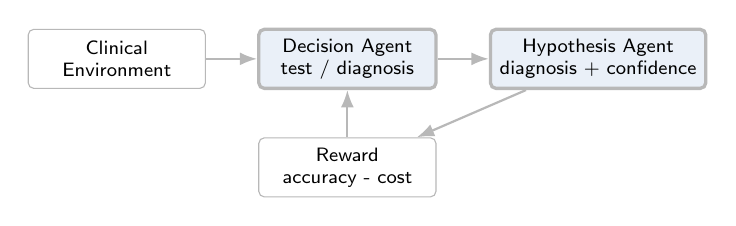
\begin{tikzpicture}[
  box/.style={draw=LineGray, rounded corners=2pt, fill=white, align=center, minimum width=2.25cm, minimum height=0.75cm, font=\scriptsize},
  train/.style={box, draw=LineGray, very thick, fill=SoftOrange},
  arr/.style={-{Latex[length=2.2mm]}, thick, draw=LineGray}
]
\node[box] (env) {Clinical\\Environment};
\node[train, right=0.65cm of env] (da) {Decision Agent\\test / diagnosis};
\node[train, right=0.65cm of da] (ha) {Hypothesis Agent\\diagnosis + confidence};
\node[box, below=0.6cm of da] (reward) {Reward\\accuracy - cost};
\draw[arr] (env) -- (da);
\draw[arr] (da) -- (ha);
\draw[arr] (ha) -- (reward);
\draw[arr] (reward) -- (da);
\end{tikzpicture}
\end{center}

\vspace{0.35em}
\begin{columns}[T,onlytextwidth]
\begin{column}{0.48\textwidth}
\begin{block}{Cyclic training objectives}
\footnotesize
\begin{enumerate}
  \item \textbf{Hypothesis generation}\\
  SFT trains HA to generate the ground-truth diagnosis \(y_{\mathrm{true}}\) at each state.
  \item \textbf{Uncertainty-awareness}\\
  GRPO calibration aligns confidence with \(J(h_j)=\mathbb{1}[h_j=y_{\mathrm{true}}]\).
  \item \textbf{Efficient action selection}\\
  GRPO trains DA to request useful tests and decide when to stop/diagnose.
\end{enumerate}
\end{block}
\end{column}
\begin{column}{0.48\textwidth}
\begin{block}{DA phase reward}
\small
\[
R_{\mathrm{diag}}=
\begin{cases}
r_{\mathrm{pos}} & y_{\mathrm{pred}}=y_{\mathrm{true}}\\
r_{\mathrm{neg}} & y_{\mathrm{pred}}\neq y_{\mathrm{true}}\\
r_{\mathrm{invalid}} & \text{format error}
\end{cases}
\]
\vspace{-0.4em}
\[
R_{\mathrm{cost}}(T)=-\sum_{t_j\in T}c(t_j)
\]
\vspace{-0.1em}
\footnotesize
This reward is used only in the \textbf{efficient action selection phase}. Hypothesis SFT and confidence calibration use separate objectives and are alternated within the training cycle.
\end{block}
\end{column}
\end{columns}
\end{frame}

\begin{frame}[t]{LA-CDM: Results and Implications}
\centering
\vspace{0.7em}
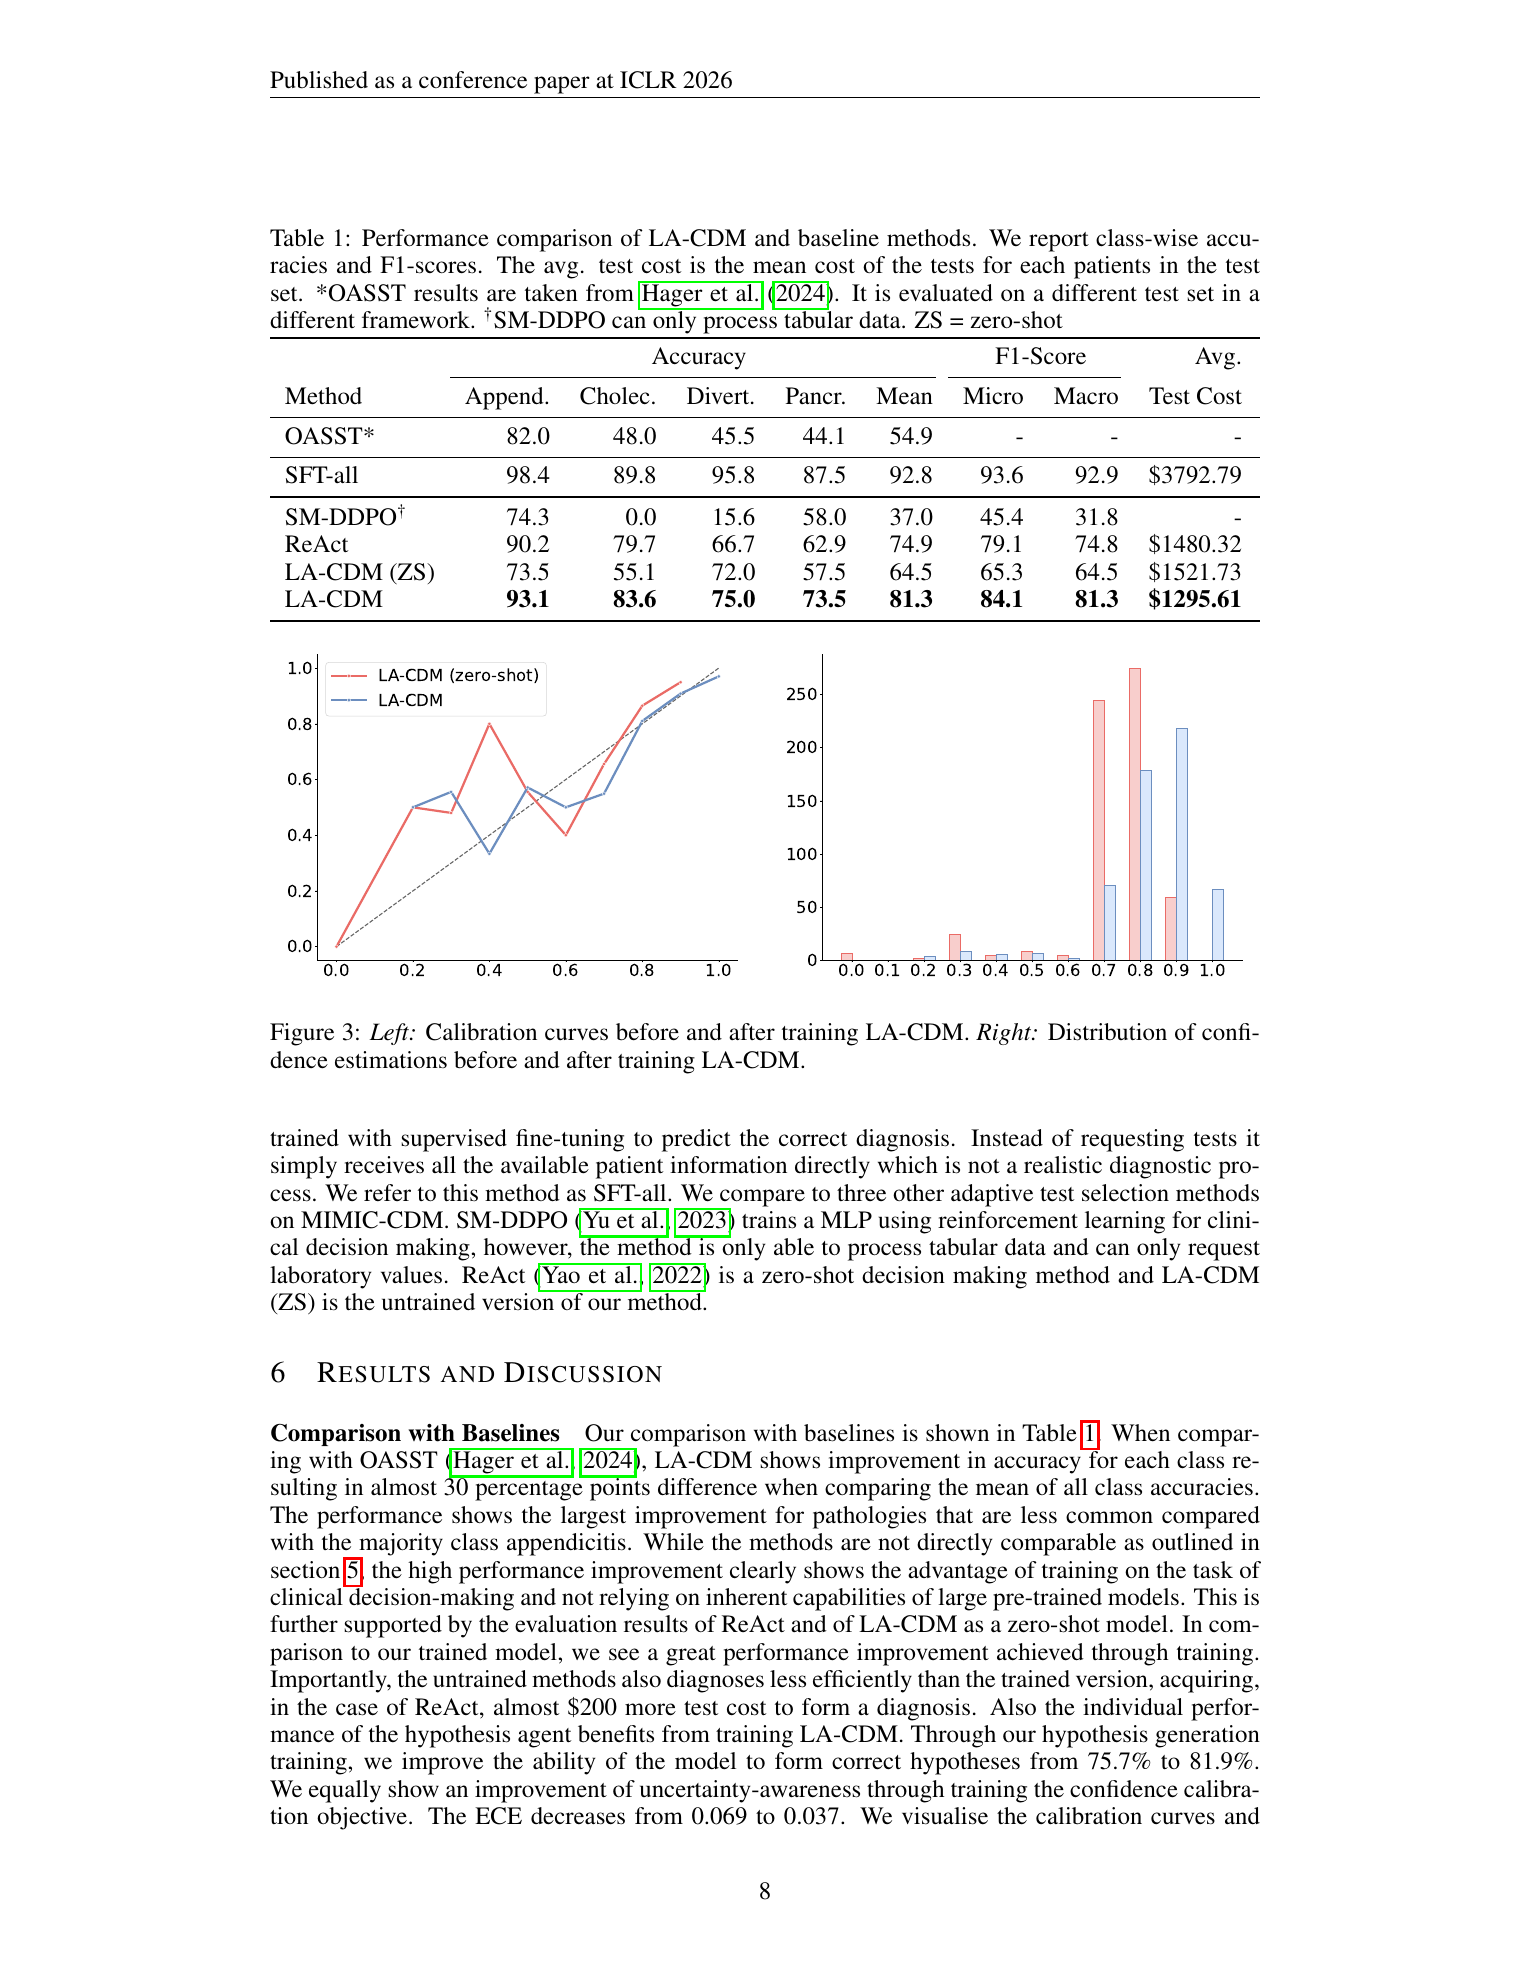
\includegraphics[
  width=0.96\linewidth,
  height=0.58\textheight,
  keepaspectratio,
  trim=3.2cm 14.0cm 2.6cm 4.9cm,
  clip
]{figures/LA-CDM/results/page-08.png}

\vspace{0.2em}
\begin{block}{What the Results Suggest}
\small
\begin{itemize}
  \item LA-CDM mean accuracy \(81.3\), macro F1 \(81.3\)
  \item Higher performance and lower average test cost than ReAct
  \item Confidence calibration also improves after training
\end{itemize}
\end{block}
\end{frame}

\begin{frame}[plain]
\centering
\vspace{0.22\textheight}
{\Large\bfseries Uncertainty-Guided Latent Diagnostic\\Trajectory Learning for Sequential Clinical Diagnosis}
\vspace{1.2em}

{\small LDTL}\\
{\scriptsize arXiv 2026}
\end{frame}

\begin{frame}{LDTL: Motivation}
\vspace{0.1em}
\begin{block}{Terminal reward is insufficient for trajectory learning}
\small
Optimizing performance and cost only through terminal reward does not directly control the \textbf{structure or distribution of diagnostic trajectories}. This can be unstable with limited clinical trajectories and provides weak supervision for desirable paths.
\end{block}

\vspace{0.55em}
\begin{center}
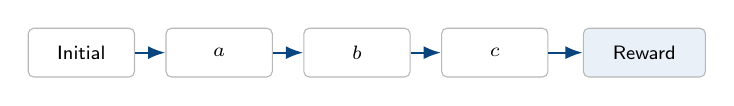
\begin{tikzpicture}[
  tnode/.style={draw=LineGray, rounded corners=2pt, fill=white, align=center, minimum width=1.35cm, minimum height=0.62cm, font=\scriptsize},
  tarrow/.style={-{Latex[length=2.2mm]}, thick, draw=AccentOrange}
]
\node[tnode] (s) at (0,0) {Initial};
\node[tnode] (a) at (1.75,0) {\(a\)};
\node[tnode] (b) at (3.50,0) {\(b\)};
\node[tnode] (c) at (5.25,0) {\(c\)};
\node[tnode, fill=SoftOrange, minimum width=1.55cm] (r) at (7.15,0) {Reward};

\draw[tarrow] (s) -- (a);
\draw[tarrow] (a) -- (b);
\draw[tarrow] (b) -- (c);
\draw[tarrow] (c) -- (r);
\end{tikzpicture}
\end{center}

\vspace{0.45em}
\begin{block}{LDTL Problem Setting}
\small
LDTL formulates test selection as a \textbf{Latent Diagnostic Trajectory Learning} problem and constructs action signals based on diagnostic improvement rather than simple rewards.
\end{block}
\end{frame}

\begin{frame}[t]{LDTL: Main Figure}
\centering
\vspace{0.35em}

\includegraphics[width=0.98\linewidth,height=0.62\textheight,keepaspectratio]{figures/LDTL/main.png}

\vspace{0.35em}
\begin{block}{Agent Roles}
\small
\textbf{Planning LLM agent}: selects the next diagnostic action based on the current patient state.

\vspace{0.2em}
\textbf{Diagnostic LLM agent}: predicts the disease label and confidence after new evidence is added.
\end{block}
\end{frame}

\begin{frame}[t]{LDTL: ideal vs. approximation}
\vspace{0.85em}
\begin{columns}[T,onlytextwidth]
\begin{column}{0.48\textwidth}
{\large\bfseries\textcolor{primary}{Ideal: trajectory posterior}}

\vspace{0.25em}
{\small
\[
q(z \mid h_0, y) =
\frac{\exp(\beta S(z))}
{\sum_{z' \in Z(h_0)} \exp(\beta S(z'))}
\]
\[
q(a_t \mid h_t, y) =
\sum_{z:z_t=a_t} q(z \mid h_0, y)
\]
}

\vspace{-0.55em}
\begin{center}
\scriptsize
\begin{tabular}{lcc}
\toprule
trajectory \(z\) & \(S(z)\) & \(q(z)\) \\
\midrule
\((A,B,C)\) & 3.0 & 0.30 \\
\((A,C,B)\) & 2.0 & 0.12 \\
\((B,A,C)\) & 2.5 & 0.20 \\
\((B,C,A)\) & 3.5 & 0.35 \\
\((C,A,B)\) & 1.0 & 0.02 \\
\((C,B,A)\) & 0.5 & 0.01 \\
\bottomrule
\end{tabular}
\end{center}

\vspace{-0.45em}
{\small
\[
q(A)=0.42,\quad q(B)=0.55,\quad q(C)=0.03
\]
}

{\scriptsize A posterior is formed from the full trajectory score \(S(z)\), then probabilities of trajectories starting with the same action are aggregated to obtain the action posterior.}
\end{column}

\begin{column}{0.02\textwidth}
\centering
\vspace{0.05em}
\rule{0.4pt}{0.70\textheight}
\end{column}

\begin{column}{0.48\textwidth}
{\large\bfseries\textcolor{primary}{Approx.: one-step IG}}

\vspace{0.25em}
{\small
\[
IG(h_0,a)=\log p(y\mid h_0+a)-\log p(y\mid h_0)
\]
\[
q(a\mid h_0,y)\propto \exp(IG(h_0,a)/\tau)
\]
}

\vspace{-0.35em}
\begin{center}
\scriptsize
\begin{tabular}{lc}
\toprule
action & one-step IG \\
\midrule
\(A\) & 0.70 \\
\(B\) & 0.50 \\
\(C\) & 0.10 \\
\bottomrule
\end{tabular}
\end{center}

\vspace{0.15em}
{\small
\[
IG(A)>IG(B)>IG(C)
\]
}

{\scriptsize In practice, training does not enumerate full trajectories. Instead, it forms the action posterior from the diagnostic improvement obtained by adding one action to the current state.}
\end{column}
\end{columns}
\end{frame}

\begin{frame}{LDTL: Method}
\vspace{0.05em}
\begin{block}{Stage 1. Train the diagnostic LLM first}
\small
The diagnostic LLM is SFT-trained to predict the correct disease label and output a confidence score when full patient information, i.e., complete diagnostic results, is provided.
\end{block}

\vspace{0.45em}
\begin{block}{Stage 2. Freeze the diagnostic LLM and train the planner}
\small
After freezing the trained diagnostic LLM, the planning LLM learns which diagnostic action to select. At each step, candidate actions are evaluated, an action-level posterior \(q(a_t\mid h_t,y)\) is constructed from \textbf{diagnostic improvement}, and the planner policy is aligned to it.
\end{block}

\vspace{0.35em}
\[
\mathcal{L}_{\mathrm{planner}}
=
\sum_{t=1}^{T}
\mathrm{KL}\!\left(q(a\mid h_t,y)\,\|\,\pi_\theta(a\mid h_t)\right)
\]

\vspace{0.15em}
\begin{block}{Key Point}
\small
Instead of constructing ground-truth trajectories directly, LDTL uses \textbf{probability changes from the frozen diagnostic LLM} to create planner supervision.
\end{block}
\end{frame}

\begin{frame}[t]{LDTL: Results and Implications}
\centering
\vspace{1.05em}
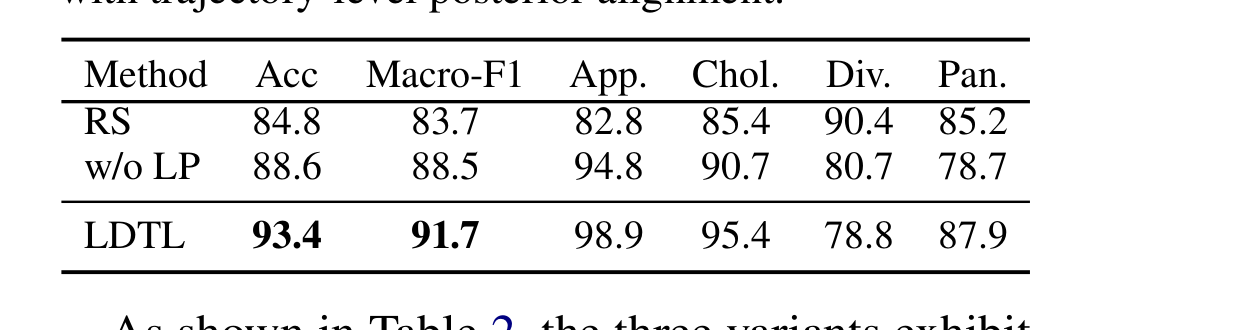
\includegraphics[
  width=0.86\linewidth,
  height=0.27\textheight,
  keepaspectratio,
  trim=0 0.25cm 0 0.45cm,
  clip
]{figures/LDTL/results/table2_crop.png}

\vspace{0.55em}
\begin{columns}[T,onlytextwidth]
\begin{column}{0.58\textwidth}
\centering
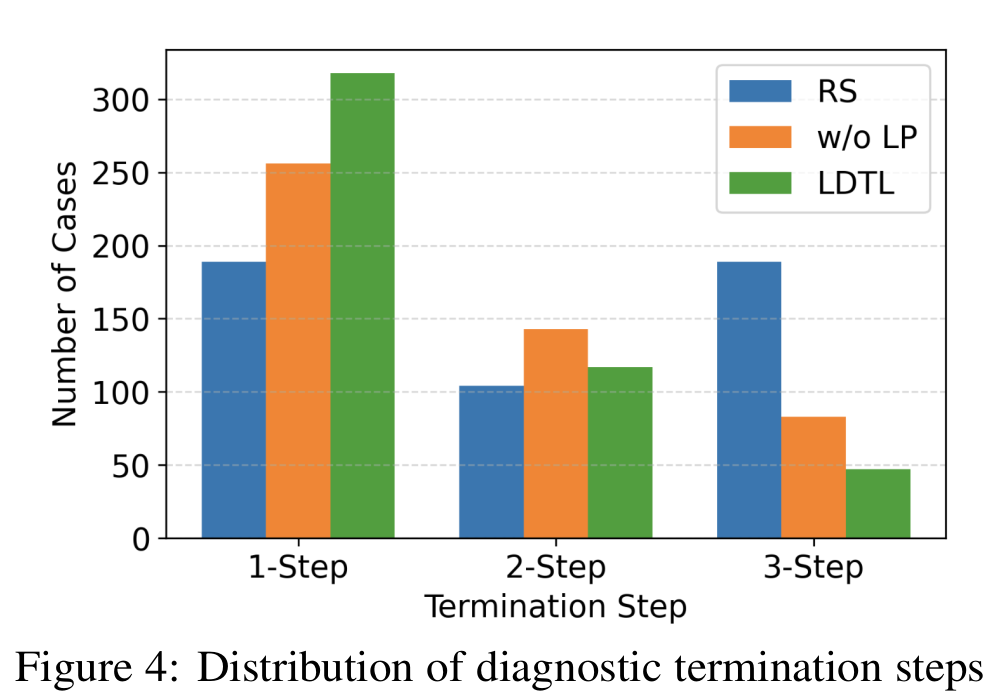
\includegraphics[
  width=0.98\linewidth,
  height=0.46\textheight,
  keepaspectratio,
  trim=0 0 0 0,
  clip
]{figures/LDTL/results/fig4_crop.png}
\end{column}

\begin{column}{0.38\textwidth}
\vspace{0.13\textheight}
\begin{block}{Interpretation}
\small
\textbf{Table 2:} LDTL outperforms RS and w/o LP in Acc and Macro-F1. This suggests that latent trajectory supervision improves final diagnostic performance.

\vspace{0.55em}
\textbf{Figure 4:} LDTL has more 1-step terminations and fewer 3-step terminations. This suggests that it learns to gather necessary information earlier and reduce unnecessary extra tests.
\end{block}
\end{column}
\end{columns}
\end{frame}

\begin{frame}[plain]
\centering
\vspace{0.22\textheight}
{\Large\bfseries Learning What Matters: Criticality-Guided\\Reinforcement Learning for Sequential Clinical Diagnosis}
\vspace{1.2em}

{\small SIFT}\\
{\scriptsize Preprint 2026}
\end{frame}

\begin{frame}{SIFT: Motivation}
\vspace{0.1em}
\begin{block}{1. Existing benchmarks restrict actions and diagnoses to closed spaces}
\small
AMIE, ED-Copilot, and LA-CDM-style benchmarks restrict the action space to a predefined test menu and the diagnosis space to a fixed label set. Real clinical reasoning, however, is closer to open-ended interaction.
\end{block}

\vspace{0.45em}
\begin{block}{2. Terminal reward does not capture evidence quality}
\small
It tells whether the final diagnosis is correct, but not whether the trajectory collected good evidence. As a result, the policy may fail to distinguish critical findings from noise and drift toward \textbf{indiscriminate information acquisition}.
\end{block}

\vspace{0.45em}
\begin{block}{SIFT Problem Setting}
\small
Instead of directly constructing ground-truth paths, SIFT turns how much \textbf{critical evidence} a trajectory retrieves into a reward signal.
\end{block}
\end{frame}

\begin{frame}[t]{SIFT: Main Figure}
\centering
\vspace{0.25em}

\includegraphics[width=0.98\linewidth,height=0.62\textheight,keepaspectratio]{figures/SIFT/main.png}

\vspace{0.35em}
\begin{block}{Components}
\small
\textbf{Critical evidence scorer}: marks diagnosis-relevant evidence at the sentence level.

\vspace{0.2em}
\textbf{Reward shaping}: converts critical evidence retrieval into intermediate rewards for learning test selection.
\end{block}
\end{frame}

\begin{frame}{SIFT: Offline Criticality Scoring}
\vspace{0.1em}
\begin{columns}[T,onlytextwidth]
\begin{column}{0.45\textwidth}
\makebox[\linewidth][r]{%
  
\includegraphics[width=1.18\linewidth,height=0.80\textheight,keepaspectratio]{figures/SIFT/image.png}%
}
\end{column}
\begin{column}{0.51\textwidth}
\vspace{0.4em}
{\large\bfseries\textcolor{primary}{1. Fact extraction}}

\vspace{0.35em}
{\small Before training, atomic clinical facts are extracted from the patient record \(M\).}

\vspace{0.15em}
{\small \(F=\phi(M)=\{f_1,\ldots,f_n\}\)}

\vspace{0.25em}
{\footnotesize Each \(f_i\) is a single observation, such as a lab value, imaging finding, or physical exam result, without mixed interpretation.}

\vspace{1.0em}
{\large\bfseries\textcolor{primary}{2. Criticality scoring}}

\vspace{0.35em}
{\small \(w_f=\psi(f\mid d^{*},o_0),\quad w_f\in\{0,1,2,3\}\)}

\vspace{0.25em}
{\footnotesize Each fact is scored by how strongly it confirms the diagnosis, conditioned on the gold diagnosis \(d^{*}\) and initial presentation \(o_0\).}

\vspace{1.0em}
{\large\bfseries\textcolor{primary}{Score meaning}}

\vspace{0.25em}
{\footnotesize
\begin{itemize}
  \item \(0\): irrelevant to the diagnosis
  \item \(1\): supportive but non-specific evidence
  \item \(2\): significant evidence
  \item \(3\): hallmark / pathognomonic finding
\end{itemize}
Scoring is performed offline, so \(\psi\) is not called during rollout.
}
\end{column}
\end{columns}
\end{frame}

\begin{frame}{SIFT: Method}
\vspace{0.35em}
{\large\bfseries\textcolor{primary}{1. Why is terminal reward insufficient?}}

\vspace{0.35em}
{\small
A binary reward that only checks whether the final diagnosis is correct is observed only at the end of the episode. It does not indicate which action contributed to the correct diagnosis, so the agent may broadly collect diagnostically irrelevant information.
}

\vspace{1.0em}
\begin{columns}[T,onlytextwidth]
\begin{column}{0.48\textwidth}
{\large\bfseries\textcolor{primary}{2. Critical recall}}

\vspace{0.35em}
{\small
Measures the fraction of critical facts retrieved by the trajectory.
}
\[
CR(\tau)=
\frac{\sum_{f \in D(\tau)} w_f}
{\sum_{f \in F} w_f}
\]
\vspace{-0.25em}
{\footnotesize \(F\): full fact set, \(D(\tau)\): discovered fact set, \(w_f\): criticality score.}
\end{column}
\begin{column}{0.48\textwidth}
{\large\bfseries\textcolor{primary}{3. Criticality-weighted reward}}

\vspace{0.35em}
{\small
The reward combines diagnostic correctness and critical evidence retrieval.
}
\[
\resizebox{\linewidth}{!}{$
R(\tau)=
\underbrace{(\alpha CR(\tau)+\beta)\,\mathrm{acc}(\hat d,d^{*})}_{\text{\scriptsize correctness reward}}
+
\underbrace{\eta CR(\tau)}_{\text{\scriptsize partial credit}}
-
\underbrace{\lambda\frac{t}{T}}_{\text{\scriptsize step penalty}}
$}
\]
\vspace{-0.45em}
{\footnotesize
\begin{itemize}
  \item \textbf{Correctness reward}: if correct, base reward \(\beta\) plus \(\alpha CR(\tau)\); if incorrect, this term is \(0\)
  \item \textbf{Partial credit}: even if incorrect, retrieving critical evidence gives \(\eta CR(\tau)\)
  \item \textbf{Step penalty}: penalizes using more test steps. \(t\): used steps, \(T\): maximum steps
\end{itemize}
}
\end{column}
\end{columns}
\end{frame}

\begin{frame}{Existing Trajectory-Level Approaches}
\vspace{0.0em}
\centering
\begin{tikzpicture}[scale=1.13, transform shape,
  node/.style={draw=LineGray, rounded corners=2pt, align=center, minimum width=1.72cm, minimum height=1.02cm, font=\scriptsize, fill=white},
  wide/.style={node, minimum width=2.35cm},
  tag/.style={font=\scriptsize\bfseries, text=primary},
  edge/.style={-{Latex[length=2.3mm]}, thick, draw=LineGray},
  note/.style={font=\scriptsize, text=TextGray, align=center}
]
\node[tag, anchor=east] at (-5.25,1.45) {LDTL};
\node[node] (l1) at (-4.35,1.45) {\(S\)\\initial};
\node[node] (l2) at (-2.55,1.45) {\(A\)};
\node[node] (l3) at (-0.75,1.45) {\(B\)};
\node[node] (l4) at (1.05,1.45) {\(C\)};
\node[wide] (l5) at (3.2,1.45) {END\\accuracy};
\draw[edge] (l1) -- (l2);
\draw[edge] (l2) -- (l3);
\draw[edge] (l3) -- (l4);
\draw[edge] (l4) -- (l5);
\node[note] at (-0.55,0.55) {construct trajectory \(z=(A,B,C)\)};
\node[note] at (3.2,0.55) {follow final confidence /\\accuracy};

\node[tag, anchor=east] at (-5.25,-1.10) {SIFT};
\node[node] (s1) at (-4.35,-1.10) {\(S\)\\initial};
\node[node] (s2) at (-2.55,-1.10) {\(A\)\\{\tiny score \(0\)}};
\node[node] (s3) at (-0.75,-1.10) {\(B\)\\{\tiny score \(3\)}};
\node[node] (s4) at (1.05,-1.10) {\(C\)\\{\tiny score \(2\)}};
\node[wide] (s5) at (3.2,-1.10) {END\\{\scriptsize \(R(\tau)=0+3+2\)}};
\draw[edge] (s1) -- (s2);
\draw[edge] (s2) -- (s3);
\draw[edge] (s3) -- (s4);
\draw[edge] (s4) -- (s5);
\node[note] at (-1.25,-2.02) {measure how many critical facts are retrieved\\within trajectory \(\tau=\{(a_t,o_t)\}\)};
\node[font=\tiny, text=TextGray, align=center] at (3.2,-2.42) {\(R(\tau)=(\alpha CR+\beta)acc+\eta CR-\lambda t/T\)};
\end{tikzpicture}

\vspace{0.35em}
\begin{alertblock}{Shared Assumption}
\small
They implicitly treat the information provided by each test as relatively \textbf{independent}. In other words, knowing one test result is assumed not to substantially change the predictive value of adding another test.
\end{alertblock}
\end{frame}

\begin{frame}{Greedy Does Not Fail Because Intermediate Reward Is Missing}
\vspace{0.1em}
\begin{columns}[T,onlytextwidth]
\begin{column}{0.48\textwidth}
\centering
{\large\bfseries\textcolor{primary}{Example 1: same second test \(C\)}}

\vspace{0.25em}
\begin{tikzpicture}[
  node distance=1.1cm and 1.55cm,
  state/.style={draw, rounded corners=2pt, align=center, minimum width=1.55cm, minimum height=0.82cm, font=\scriptsize, fill=white},
  good/.style={draw=primary, very thick, fill=SoftOrange},
  better/.style={draw=secondary, very thick, fill=secondary!8},
  edge/.style={->, thick},
  gre/.style={->, very thick, primary},
  alt/.style={->, very thick, secondary}
]
\node[state] (s) {Initial\\\(U=0.00\)};
\node[state, good, below left=of s] (a) {\(A\)\\\(U=0.70\)};
\node[state, below right=of s] (b) {\(B\)\\\(U=0.50\)};
\node[state, below=of a] (ac) {\(A+C\)\\\(U=0.71\)};
\node[state, better, below=of b] (bc) {\(B+C\)\\\(U=0.80\)};
\draw[gre] (s) -- node[above left, font=\scriptsize] {\(A\)} (a);
\draw[edge] (s) -- node[above right, font=\scriptsize] {\(B\)} (b);
\draw[edge] (a) -- node[left, font=\scriptsize] {\(+C\)} (ac);
\draw[alt] (b) -- node[right, font=\scriptsize] {\(+C\)} (bc);
\end{tikzpicture}

\vspace{0.25em}
{\footnotesize
Greedy selects \(A\) because \(U(A)>U(B)\). But when the same \(C\) is added, \(B+C\) becomes better.
}
\end{column}
\begin{column}{0.48\textwidth}
\centering
{\large\bfseries\textcolor{primary}{Example 2: different second test}}

\vspace{0.25em}
\begin{tikzpicture}[
  node distance=1.1cm and 1.55cm,
  state/.style={draw, rounded corners=2pt, align=center, minimum width=1.55cm, minimum height=0.82cm, font=\scriptsize, fill=white},
  good/.style={draw=primary, very thick, fill=SoftOrange},
  better/.style={draw=secondary, very thick, fill=secondary!8},
  edge/.style={->, thick},
  gre/.style={->, very thick, primary},
  alt/.style={->, very thick, secondary}
]
\node[state] (s2) {Initial\\\(U=0.00\)};
\node[state, good, below left=of s2] (a2) {\(A\)\\\(U=0.70\)};
\node[state, below right=of s2] (b2) {\(B\)\\\(U=0.50\)};
\node[state, below=of a2] (ac2) {\(A+C\)\\\(U=0.72\)};
\node[state, better, below=of b2] (bd2) {\(B+D\)\\\(U=0.82\)};
\draw[gre] (s2) -- node[above left, font=\scriptsize] {\(A\)} (a2);
\draw[edge] (s2) -- node[above right, font=\scriptsize] {\(B\)} (b2);
\draw[edge] (a2) -- node[left, font=\scriptsize] {\(+C\)} (ac2);
\draw[alt] (b2) -- node[right, font=\scriptsize] {\(+D\)} (bd2);
\end{tikzpicture}

\vspace{0.25em}
{\footnotesize
At first, \(A\) looks better, but \(B\) creates a higher trajectory utility when paired with \(D\).
}
\end{column}
\end{columns}

\vspace{0.25em}
\begin{alertblock}{Takeaway}
\small
Even with intermediate rewards, evaluating \(A\) and \(B\) independently makes \(A\) look better. The issue is not where the reward is placed, but that the value of one test depends on \textbf{which later tests it is combined with}.
\end{alertblock}
\end{frame}

\begin{frame}{So What Can We Do?}
\vspace{0.25em}

\begin{columns}[T,onlytextwidth]
\begin{column}{0.48\textwidth}
\begin{block}{1. Bayesian network}
\small
\textbf{Description}\\
Explicitly models conditional dependencies between tests and updates the posterior as evidence is added.

\vspace{0.55em}
\textbf{Pros}
\begin{itemize}
  \item Can handle combination effects and redundancy in principle
  \item Can define query order probabilistically
\end{itemize}

\vspace{0.25em}
\textbf{Cons}
\begin{itemize}
  \item Hard to convert natural-language reports into discrete variables
  {\scriptsize e.g., CT report \(\rightarrow\) severe: yes/no reduces expressiveness}
\end{itemize}
\end{block}
\end{column}

\begin{column}{0.48\textwidth}
\begin{block}{2. \(n\)-step lookahead training}
\small
\textbf{Description}\\
Instead of evaluating only the current test, measure the utility of possible \(n\)-step combinations ahead and use it as a learning signal.

\vspace{0.45em}
\textbf{Pros}
\begin{itemize}
  \item Does not require labeling all subsets
  \item Can directly teach synergy in small combinations
\end{itemize}

\vspace{0.2em}
\textbf{Cons}
\begin{itemize}
  \item Computational cost grows exponentially
\end{itemize}

\vspace{0.15em}
\centering
{\scriptsize
\begin{tabular}{r r r}
\toprule
Max step & Subsets & Coverage \\
\midrule
1 & 12 & 0.29\% \\
2 & 78 & 1.90\% \\
3 & 298 & 7.28\% \\
4 & 793 & 19.37\% \\
5 & 1,585 & 38.71\% \\
6 & 2,509 & 61.27\% \\
7 & 3,301 & 80.61\% \\
8 & 3,796 & 92.70\% \\
\bottomrule
\end{tabular}
}
\end{block}
\end{column}
\end{columns}
\end{frame}

\begin{frame}[plain]
\centering
\vfill
{\Huge\bfseries Thank You}
\vfill
\end{frame}

\end{document}
